\section{Architecture}\label{sec:architecture}

The Åboat already has an architecture of its own. The system is already functional (though it has its own communication protocol). What we aim to do is build on top of this architecture.
\\\\
Currently, the Åboat has an architecture that consists of microservices. Each of these microservices runs a different “functionality” of the boat. There are microservices for sensors, control, storage, and communication. The current picture of the Åboat architecture can be seen in the image below. Our microservice, the one implementing the VRGP specification and responsible for message exchange with a MOC on the shore, will probably be connected to every other microservice on the boat - especially important are the sensor microservices. As such, the microservice will play an essential role in the architecture of the Åboat.
\\\\
Note however, that our microservice will not replace existing communication microservices, but will instead run along with them.
\\\\
The microservice will consist of two high level-view modules: one module will be a generic VRGP implementation (not Åboat related), which will take care of the communication with the MOC on the shore, and one module will be in charge of talking with the other microservices on the boat that provide sensor data. The role of the first module will be that of a communicator, while the role of the second module will thus be that of a data aggregator.

\begin{figure}[ht]
	\centering
	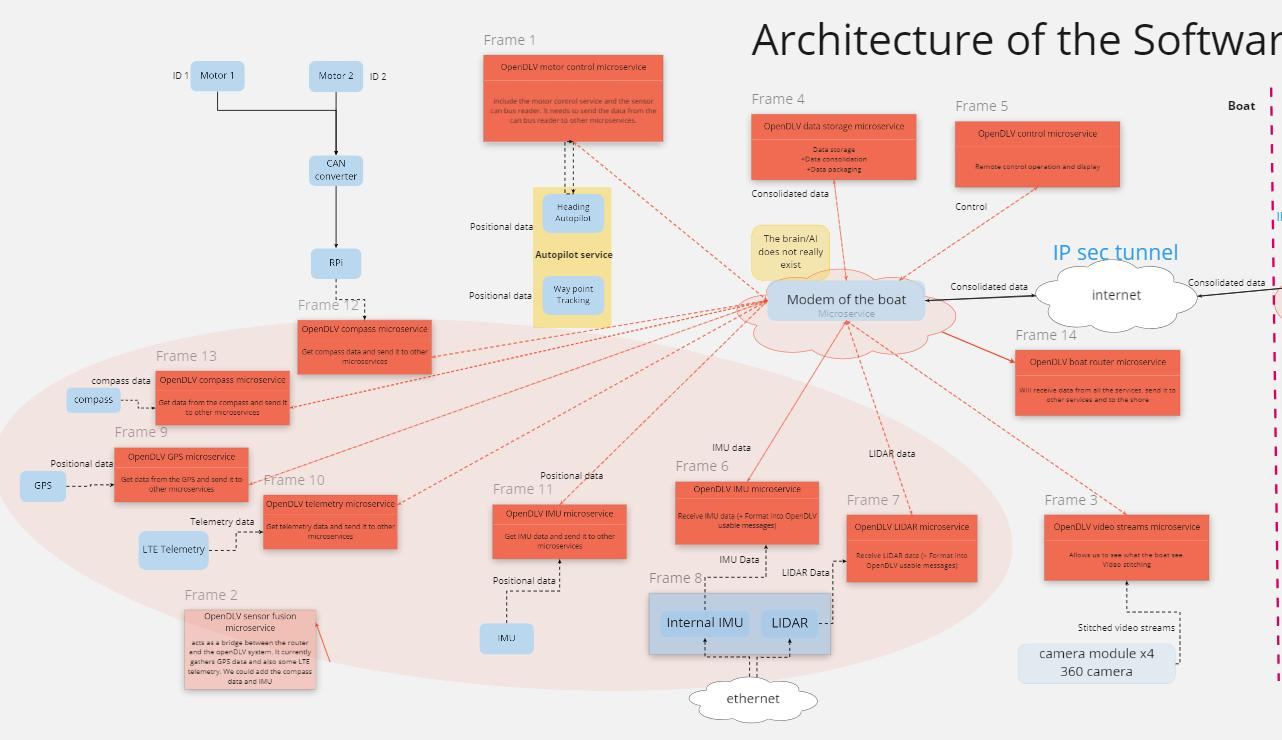
\includegraphics[width=\linewidth]{images/aboat-architecture}
	\caption{Åboat architecture}
	\label{fig:aboat-architecture}
\end{figure}

\section{Design}\label{sec:design}

In the following sections, we describe our initial design using several UML diagrams. UML is used for most parts of the design for now, as it provides a well-known, easy to understand and somewhat unambiguous description of the design. For now, the diagrams depict rather high-level views of the system. In further design steps, the diagrams will be refined and more specific diagram types will be added to the design. Before entering the next refinement stage, the design is always presented to and agreed upon with the customers.

\subsection{Static Design}

\subsubsection{Deployment Diagram}

The deployment diagram provides an overview of the different deliverables for this software project and in which environments they can be used. The most important artifact to be delivered is the OpenDLV microservice for the Åboat which is embedded in the Åboat environment. Additionally, an MOC example implementation will be developed to test the VRGP implementation for the Åboat. This consists of a backend and a frontend to make testing easy for us and future users.

\begin{figure}[ht]
	\centering
	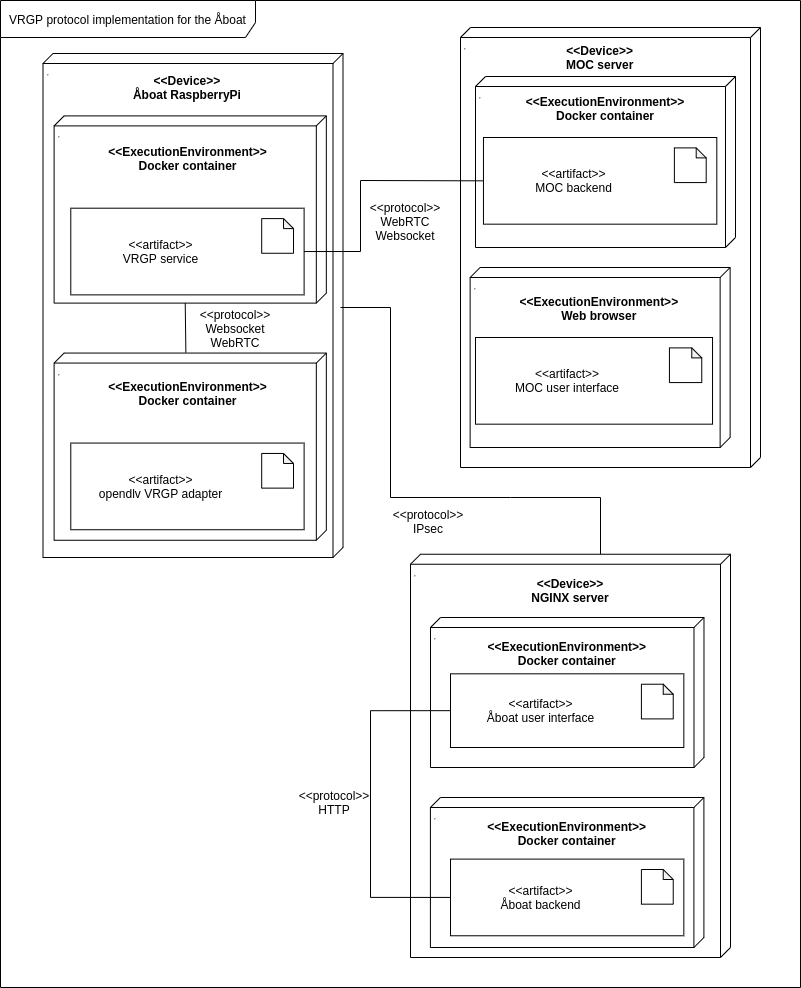
\includegraphics[width=\linewidth]{diagrams/deployment-diagram}
	\caption{Deployment diagram}
	\label{fig:deployment-diagram}
\end{figure}

\subsubsection{Component Diagram}

The next step in the design process will be the development of a component diagram for our software. This will divide the software into components, somewhat according to the use cases and requirements (see \ref{sec:func-requirements}), and define which components communicate with each other in what form. The component diagram will be the basis for further, more detailed design steps such as class diagrams.

\subsection{Dynamic Design}\label{sec:dynamic-design}

\subsubsection{Activity Diagram}

This high-level activity diagram provides an overview of the general communication flow in the VRGP protocol, including the connection establishment and authentication, the messages that can be sent continuously while the connection is up and the termination of the connection. In further steps, this diagram will either be refined to account for more details of the protocol or split into multiple activity diagrams to depict the different processes in more detail.

\begin{figure}[ht]
	\centering
	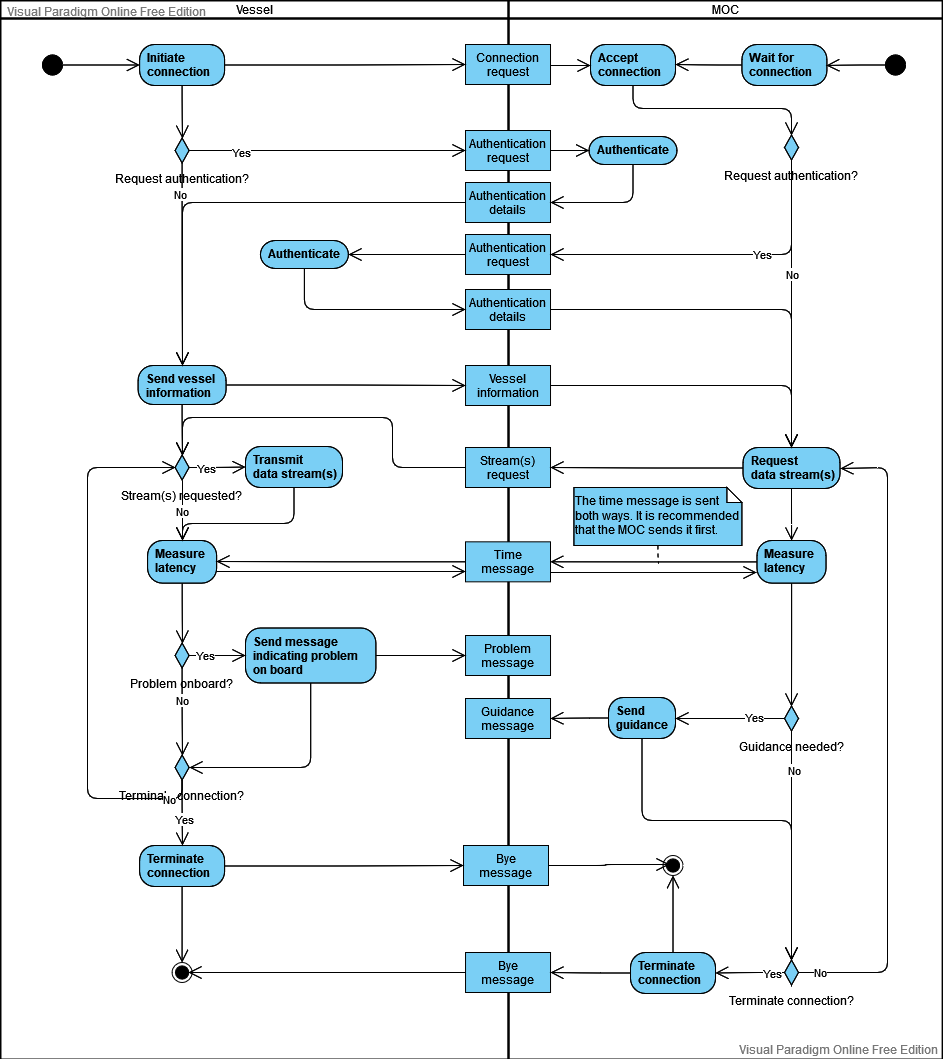
\includegraphics[width=\linewidth]{diagrams/activity-diagram}
	\caption{Activity diagram}
	\label{fig:activity-diagram}
\end{figure}

\subsubsection{Sequence Diagram}

In another design refinement step, sequence diagrams for different processes and sub-processes will be developed to clearly define the communication flow and how it will be implemented in the software using the components and classes we defined in \ref{sec:dynamic-design}.
